% \documentclass{fp-slides}
\documentclass[10pt,portrait]{beamer}
\usepackage{mathtext}
\usetheme{Warsaw}
\newcommand{\maybepause}{}
%\newcommand{\maybepause}{\pause}
\setlength{\floatsep}{8pt plus 2pt minus 2pt}
\setlength{\textfloatsep}{8pt plus 2pt minus 2pt}
\setlength{\intextsep}{12pt plus 2pt minus 2pt}
\AtBeginDocument{%
% \selectlanguage{russian}%
\frenchspacing
\righthyphenmin=2
\sloppy
%\author{Shiray Andrey}
\institute{O.O.Bogomolets National Medical University}
\title{Biostatistics}
% Basics of statistical processing of biomedical  data
}

% \ifx\pdfoutput\undefined
% % we are running LaTeX, not pdflatex
% \usepackage{graphicx}
% \else
% % we are running pdflatex, so convert .eps files to .pdf
% \usepackage[pdftex]{graphicx}
% \usepackage{epstopdf}
% \fi 
\usepackage{graphics}
\begin{document}

%%%%%%%%%%%%%%% Define code blocks

% \defverbatim[colored]\factCcode{%
% \begin{lstlisting}[frame=single,language=C]
%   int fact(int n)
%   { int x = 1;
%     while (n > 0)
%      { x = x * n;
%        n = n - 1;
%      }
%     return x;
%   }
% \end{lstlisting}}
% 
% \defverbatim[colored]\factMLcode{%
% \begin{lstlisting}[frame=single]
%   let rec fact n =
%     if n = 0 then 1
%     else n * fact(n - 1);;
% \end{lstlisting}}
% 
% \defverbatim[colored]\badFuncCode{%
% \begin{lstlisting}[frame=single]
%   int rand(void)
%   { static int n = 0;
%     return n = 2147001325 * n + 715136305;
%   }
% \end{lstlisting}}

%%%%%%%%%%%%%%%%%%%%%%

\frame{\titlepage}

% \section*{Biostatistics}

%\subsection{Обсуждаемые темы}


\frame{
  \frametitle{Crash course into Probability theory}

  \begin{itemize}
  \item \Large Probability, Random variables
    \maybepause

   \item Mean and Variance
     \maybepause
   
  \item Probability density function, Probability distributions
    \maybepause

  \item Central limit theorem
    \maybepause
  \end{itemize}
}

\frame{
\frametitle{Probability}
\begin{itemize}
\item Probability
\end{itemize}

}

\frame{
\frametitle{Probability}
\begin{itemize}
\item Probability
\begin{enumerate}
\item The probability of a random event denotes the relative frequency of occurrence of an experiment's outcome, when repeating the experiment.
\item Probability is a way to represent an individual's degree of belief in a statement.
\end{enumerate}
\end{itemize}

}

\frame{
\frametitle{Probability}
\begin{itemize}
\item Probability
\begin{enumerate}
\item The probability of a random event denotes the relative frequency of occurrence of an experiment's outcome, when repeating the experiment.
\item Probability is a way to represent an individual's degree of belief in a statement.
\end{enumerate}
\item Randomness are not the same things!
\end{itemize}

}

\frame{
\frametitle{Probability, now in plain English...}
\Large
Probability is the measure of how likely an event is.

}

\frame{
\frametitle{Probability}
The theory of chance consists in reducing all the events of the same kind to a certain number of cases equally possible, that is to say, to such as we may be equally undecided about in regard to their existence, and in determining the number of cases favorable to the event whose probability is sought. The ratio of this number to that of all the cases possible is the measure of this probability, which is thus simply a fraction whose numerator is the number of favorable cases and whose denominator is the number of all the cases possible.

\textit{ -- Pierre-Simon Laplace, A Philosophical Essay on Probabilities}
}

\frame{
\frametitle{Probability, now in plain English...}
\Large
Probability is the measure of how likely an event is.
\resizebox{.6\hsize}{!}{$P(A)=\frac{\left | A \right |}{\left | \Omega  \right |}$} 
}

\frame{
\frametitle{Probability, now in plain English...}
\begin{itemize}
\item The {\bf sample space}, $\Omega$, is the collection of possible
  outcomes of an experiment 
  \begin{list}{}{}
  \item  Example: die roll $\Omega = \{1,2,3,4,5,6\}$
  \end{list}
\item An {\bf event}, say $A$, is a subset of $\Omega$ 
  \begin{list}{}{}
  \item Example: die roll is even $A = \{2,4,6\}$
  \end{list}
\item An {\bf elementary} or {\bf simple} event is a particular result
  of an experiment
  \begin{list}{}{}
  \item Example: die roll is a four, $\omega = 4$
  \end{list}
\item $\emptyset$ is called the {\bf null event} or the {\bf empty set}
\end{itemize}

}

\frame{
\frametitle{Probability, now in plain English...}
\Large
Probability is the measure of how likely an event is.
\resizebox{.6\hsize}{!}{$P(A)=\frac{\left | A \right |}{\left | \Omega  \right |}$} 
\begin{tabular}{ccc}
$\left | A \right |$ -- The number of ways event A can occur \\
$\left | \Omega  \right | $ -- The total number of possible outcomes
\end{tabular}
}

\frame{
  \frametitle{Probability}

\begin{tabular}{ccc}
\resizebox{.6\hsize}{!}{$P(A)=\frac{\left | A \right |}{\left | \Omega  \right |}$} &  \\ 
\\ 
\resizebox{.4\hsize}{!}{$ \Omega=\left \{ heads, tails \right \}$} & \resizebox{.4\hsize}{!}{$ \Omega=\left \{ 1, 2, 3, 4, 5, 6 \right \}$}\\
\resizebox{.4\hsize}{!}{$A=heads$} & \resizebox{.4\hsize}{!}{$A=\left \{ 5,6\right \}$}  \\ 
\resizebox{.4\hsize}{!}{$P(A)=\frac{\left | A \right |}{\left | \Omega  \right |} = \frac{1}{2}$ } & \resizebox{.4\hsize}{!}{$P(A)=\frac{\left | A \right |}{\left | \Omega  \right |} = \frac{2}{6}= \frac{1}{3}$ }
\end{tabular}
}

\frame{
  \frametitle{Random variables}
 \begin{itemize}
\item \textbf{Random variable} is a function, which maps events or outcomes to real numbers 


\resizebox{.2\hsize}{!}{$\xi : \Omega \to \mathbb{R}$}
\maybepause
\item A random variable's possible values might represent the possible outcomes of a yet-to-be-performed experiment, or the potential values of a quantity whose already-existing value is uncertain.  Intuitively, a random variable can be thought of as a quantity whose value is not fixed, but which can take on different values.
\maybepause

\item Example:
\[
Y(\omega) = \begin{cases}
          1, & \text{if} \ \ \omega = \text{heads} ,\\
          0, & \text{if} \ \ \omega = \text{tails} .
        \end{cases}
\]
\maybepause
\end{itemize}
}

\frame{
  \frametitle{Probability density function}
 \begin{itemize}
\item \textbf{Probability density function} of a continuous random variable is a function that describes the relative likelihood for this random variable to occur at a given point. 

\item The probability for the random variable to fall within a particular region is given by the integral of this variable’s density over the region. The probability density function is nonnegative everywhere, and its integral over the entire space is equal to one
\end{itemize}
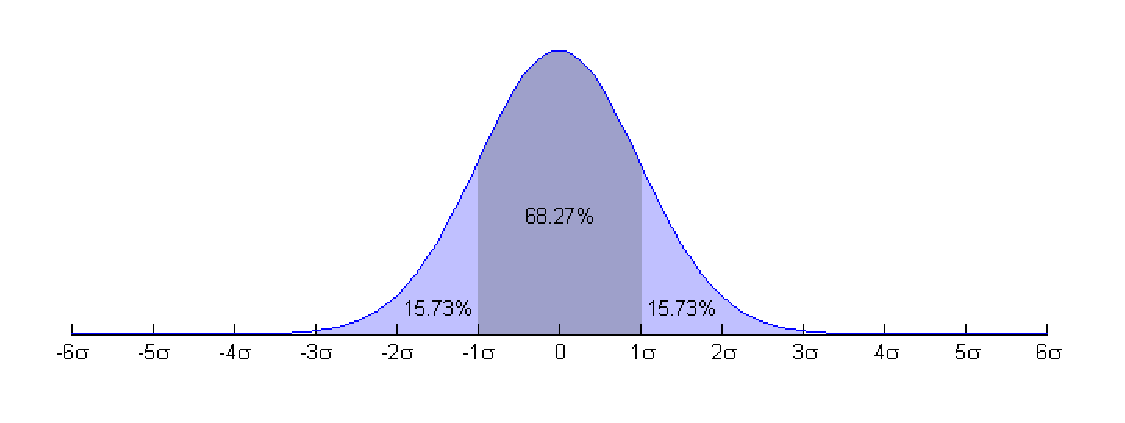
\includegraphics[scale=0.5]{den} 
}


\frame{
  \frametitle{Mathematical Expectation}
 \begin{itemize}
\item \textbf{Mathematical expectation} of a random variable is the weighted average of all possible values that this random variable can take on. The weights used in computing this average correspond to the probabilities in case of a discrete random variable, or densities in case of a continuous random variable. 

\item Discrete random variable: $\operatorname{E}[X] = \sum_{i} x_i\, p_i$

\item Continuous random variable: $\operatorname{E}[X] = \int_{-\infty}^\infty x p(x)\, \operatorname{d}x$

\item Example:

Let $X$ represent the outcome of a roll of a six-sided dice. More specifically, $X$ will be the number of pips showing on the top face of the die after the toss. The possible values for $X$ are 1, 2, 3, 4, 5, 6, all equally likely. The expectation of $X$ is
\[
    \operatorname{E}[X] = 1\cdot\frac16 + 2\cdot\frac16 + 3\cdot\frac16 + 4\cdot\frac16 + 5\cdot\frac16 + 6\cdot\frac16 = 3.5.
\]
\end{itemize}
}

\frame{
  \frametitle{Variance}
 \begin{itemize}
\item \textbf{Variance} is a measure of how far a set of numbers are spread out from each other. 

\item If a random variable $\xi$ has the \textbf{expected value} $\mu = E[\xi]$, then the variance of $\xi$ is given by:
\[
        \operatorname{Var}(\xi) = \operatorname{E}[(\xi - \mu)^2] 
\]
% =  \operatorname{E}[\xi^2] - (\operatorname{E}[\xi])^2
\item Discrete random variable: $\operatorname{Var}(X) = \sum_{i=1}^n p_i\cdot(x_i - \mu)^2 $, where $\mu = \sum_{i=1}^n p_i\cdot x_i$
\item Let $X$ represent the outcome of a roll of a six-sided dice. The variance of $X$ is
$
\sum_{i=1}^6 \tfrac{1}{6}(i - 3.5)^2 = \tfrac{1}{6}\sum_{i=1}^6 (i - 3.5)^2  = \tfrac{1}{6}\left((-2.5)^2{+}(-1.5)^2{+}(-0.5)^2{+}0.5^2{+}1.5^2{+}2.5^2\right) = \tfrac{1}{6} \cdot 17.50 = \tfrac{35}{12} \approx 2.92
$
% \[\sum_{i=1}^6 \tfrac{1}{6}(i - 3.5)^2 = \tfrac{1}{6}\sum_{i=1}^6 (i - 3.5)^2  = \tfrac{1}{6}\left((-2.5)^2{+}(-1.5)^2{+}(-0.5)^2{+}0.5^2{+}1.5^2{+}2.5^2\right) \\
%  = \tfrac{1}{6} \cdot 17.50 = \tfrac{35}{12} \approx 2.92 \]
\end{itemize}
}


\frame{
  \frametitle{Uniform distribution}

\begin{itemize}
\item Probability density function: $\begin{cases}
                  \frac{1}{b - a} & \text{for } x \in [a,b]  \\
                  0               & \text{otherwise}
                \end{cases}$
\item $\operatorname{E}[\xi]=\tfrac{1}{2}(a+b)$, $\operatorname{Var}[\xi]=\tfrac{1}{12}(b-a)^2$
\end{itemize}
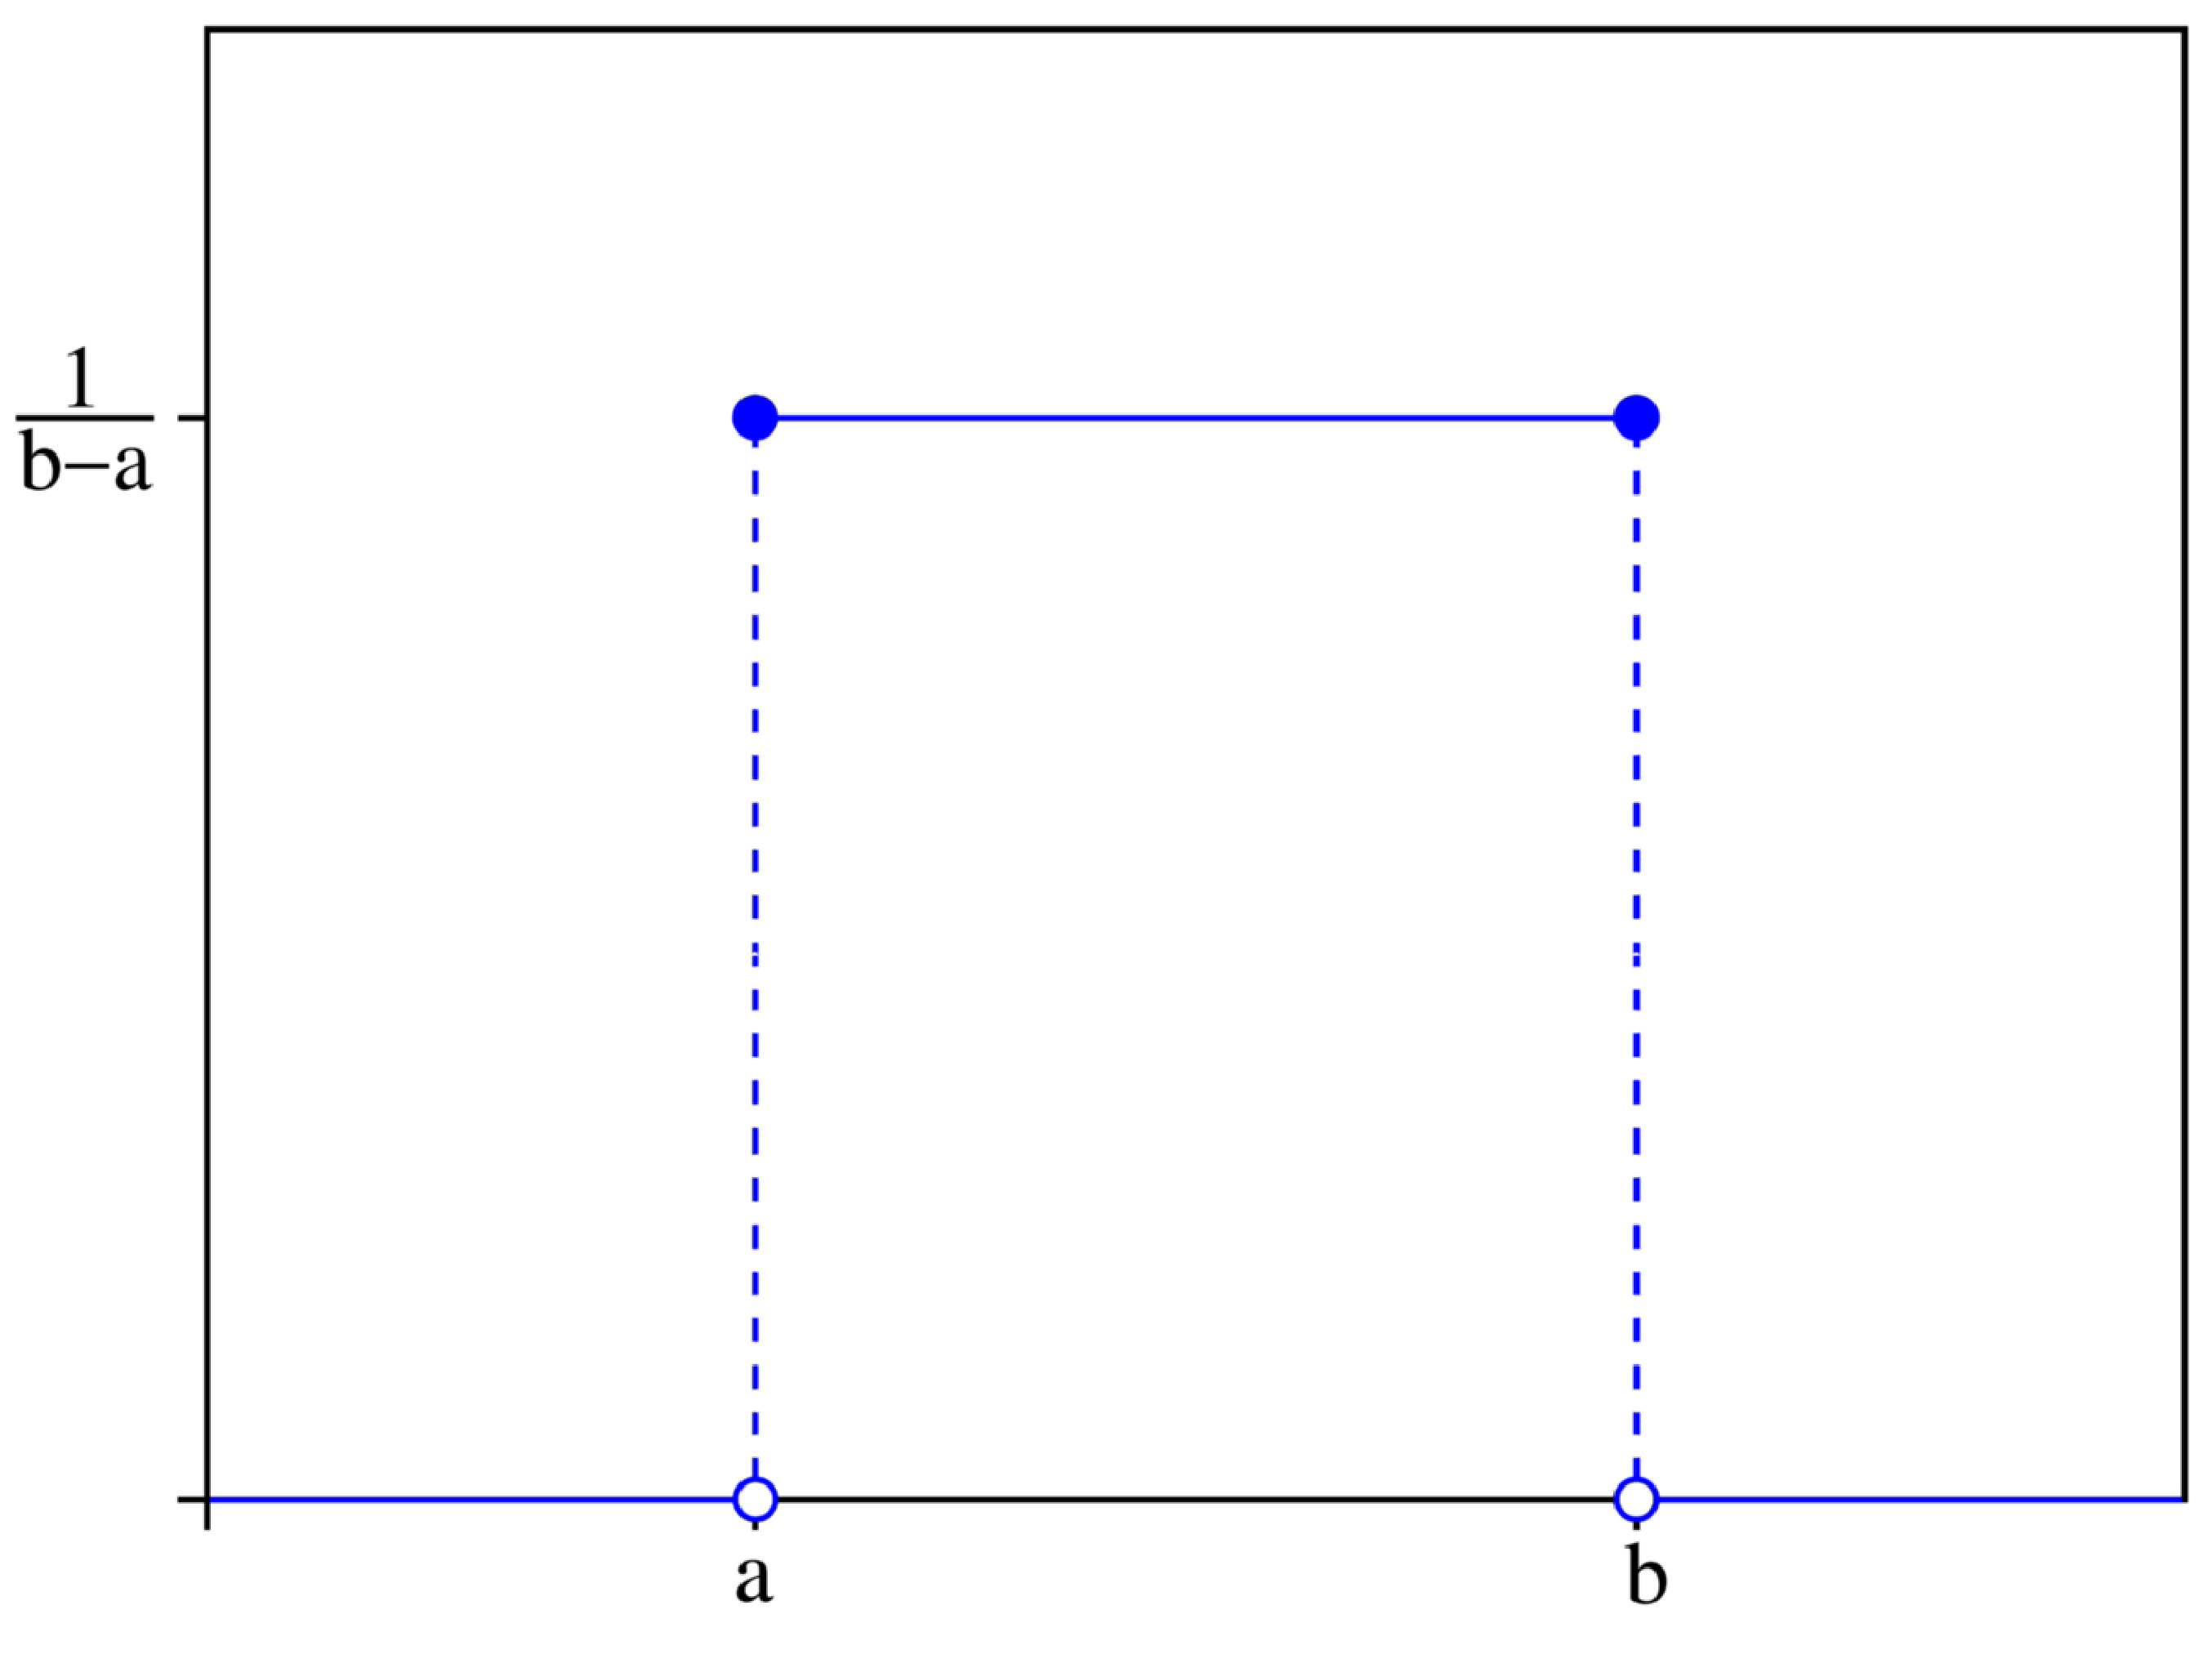
\includegraphics[scale=0.15]{uni} 
}

\frame{
  \frametitle{Poisson distribution}
\begin{itemize}
\item  Probability mass function: $p(X=k)=\frac{\lambda^k e^{-\lambda}}{k!}\!$
\item $\operatorname{E}[X]=\lambda$, $\operatorname{Var}[X]=\lambda$
\item Expresses the probability of a number of events occurring in a fixed period of time if these events occur with a known average rate and independently of the time since the last event. 
\end{itemize}
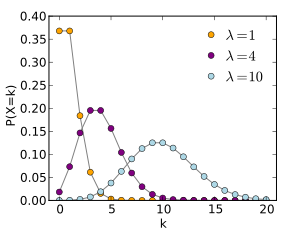
\includegraphics[scale=0.5]{pois} 
}

\frame{
  \frametitle{Normal distribution}
\begin{itemize}
\item Probability density function: $\tfrac{1}{\sqrt{2\pi\sigma^2}}\,e^{ -\frac{(x-\mu)^2}{2\sigma^2} }$
\item $\operatorname{E}[\xi]=\mu$, $\operatorname{Var}[\xi]=\sigma$

\end{itemize}
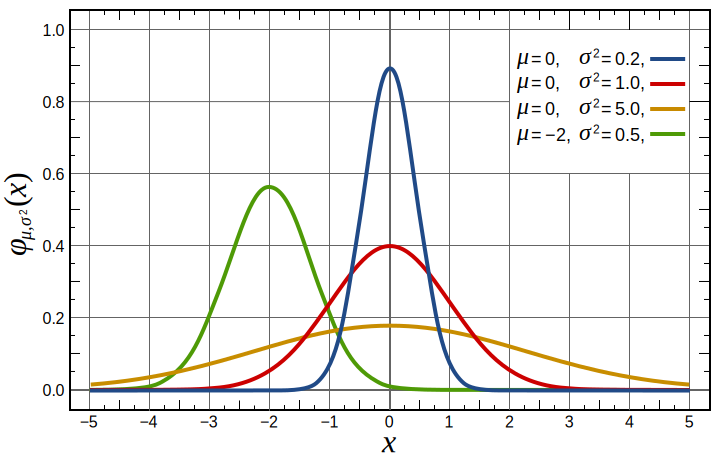
\includegraphics[scale=0.25]{norm} 

}

 \frame{
   \frametitle{Central limit theorem}
\begin{itemize}
\item 
 Conditions under which the mean of a sufficiently large number of independent\footnote{and identically distributed} random variables, each with finite mean and variance, will be approximately normally distributed. 
\[
 \frac{S_n -n\mu }{\sqrt{n}\sigma} \xrightarrow{d} N(0,1), \mu = \operatorname{E}x_i , \sigma = \operatorname{Var}x_i
\]

\item Since real-world quantities are often the balanced sum of many unobserved random events, this theorem provides a partial explanation for the prevalence of the normal probability distribution. 
\item The CLT also justifies the approximation of large-sample statistics to the normal distribution in controlled experiments.\end{itemize}

 }

% % % % % % % % % % % % % % 
%  Перерыв
% % % % % % % % % % % % % % 

\frame{
\frametitle{Break}
\Huge Let's have a \textbf{break}!


}

%%%%%%%%%%%%%%%%%%%%%%%%%%%%%%%%%%%%%%%%%%%%%%
\frame{
  \frametitle{Biostatistics}

  \begin{itemize}
  \item \Large Statistics and Biology
    \maybepause

  \item Experimental and observational studies
%    \item Random variable and Samples. Basic statistical concepts.
     \maybepause
   
  \item Sampling error
    \maybepause



  \item Correlation and Regression analysis
    \maybepause

  \item Statistical hypothesis testing
    \maybepause
  \end{itemize}
}

\frame{
  \frametitle{Statistics}
\begin{itemize}
\item \huge \textbf{Statistics} is the science of the collection, organization, and interpretation of data.

\item \normalsize It deals with all aspects of this, including the planning of data collection in terms of the design of surveys and experiments.
\item \textbf{Biostatistics} is the application of statistics to a wide range of topics in biology. The science of biostatistics encompasses the design of biological experiments, especially in medicine and agriculture; the collection, summarization, and analysis of data from those experiments; and the interpretation of, and inference from, the results.
\end{itemize}
}

\frame{
  \frametitle{Why it's important?}
\Huge Lies, damned lies, and \textbf{statistics}
}


\frame{
  \frametitle{Biostatistics}
  \begin{quote}
    Biostatistics is a theory and methodology for the acquisition
    and use of quantitative evidence in biomedical research.
    Biostatisticians develop innovative designs and analytic methods
    targeted at increasing available information, improving the
    relevance and validity of statistical analyses, making best use of
    available information and communicating relevant uncertainties.  
  \end{quote}
From the Johns Hopkins Department of Biostatistics 2007 self   study
}

\frame{
  \frametitle{Applications of biostatistics}
\begin{itemize}
\item Public health, including epidemiology, health services research, nutrition, and environmental health
\item Design and analysis of clinical trials in medicine
\item Population genetics, and statistical genetics
\item Anaysis of genomics data
\item Ecology, ecological forecasting
\item Biological sequence analysis 
\item Systems biology for gene network inference or pathways analysis

\end{itemize}
}

\frame{
  \frametitle{Random variable and Samples. Statistical Population.}
\begin{itemize}
\item A \textbf{statistical population} is a set of entities concerning which statistical inferences are to be drawn
\item \textbf{Sample} is a subset of a population
\item A sample concretely represents n experiments in which we measure the same quantity.
\item Example: 

We want to measure the height of our patients. In this case statistical population -- set of all posible heights of patient. If $X$ represents the height of an individual and we measure $N$ individuals, $X_i$ will be the height of the $i$-th individual. 
\end{itemize}
}
\frame{
  \frametitle{Sample Mean, Mode, Median. Sample Variance, Standart Deviation }
\begin{itemize}
\item \textbf{Sample Mean}: $\bar{x}=\frac{1}{N}\sum_{k=1}^{N}x_k$
\item \textbf{Mode} is the value that occurs most frequently in a data set or a probability distribution
\item \textbf{Median}  is the numeric value separating the higher half of a sample from the lower half.
\item \textbf{Sample Variance}: $\sigma_N^2 = \frac 1N \sum_{i=1}^n \left(x_i - \overline{x} \right)^ 2$
\item \textbf{Standart Deviation}: $\sigma_N = \sqrt{\frac{1}{N} \sum_{i=1}^N (x_i - \overline{x})^2}$
\end{itemize}
}
\frame{
  \frametitle{Histogram}
\[
p_{n}(x)= \sum_{k=1}^{N}\frac{1}{\left | \Delta_k \right |}v_kI_{\Delta_k}(x), v_k = \frac{1}{n}\sum_{n}^{j=1}I_{\Delta_k}(X_j)
\]
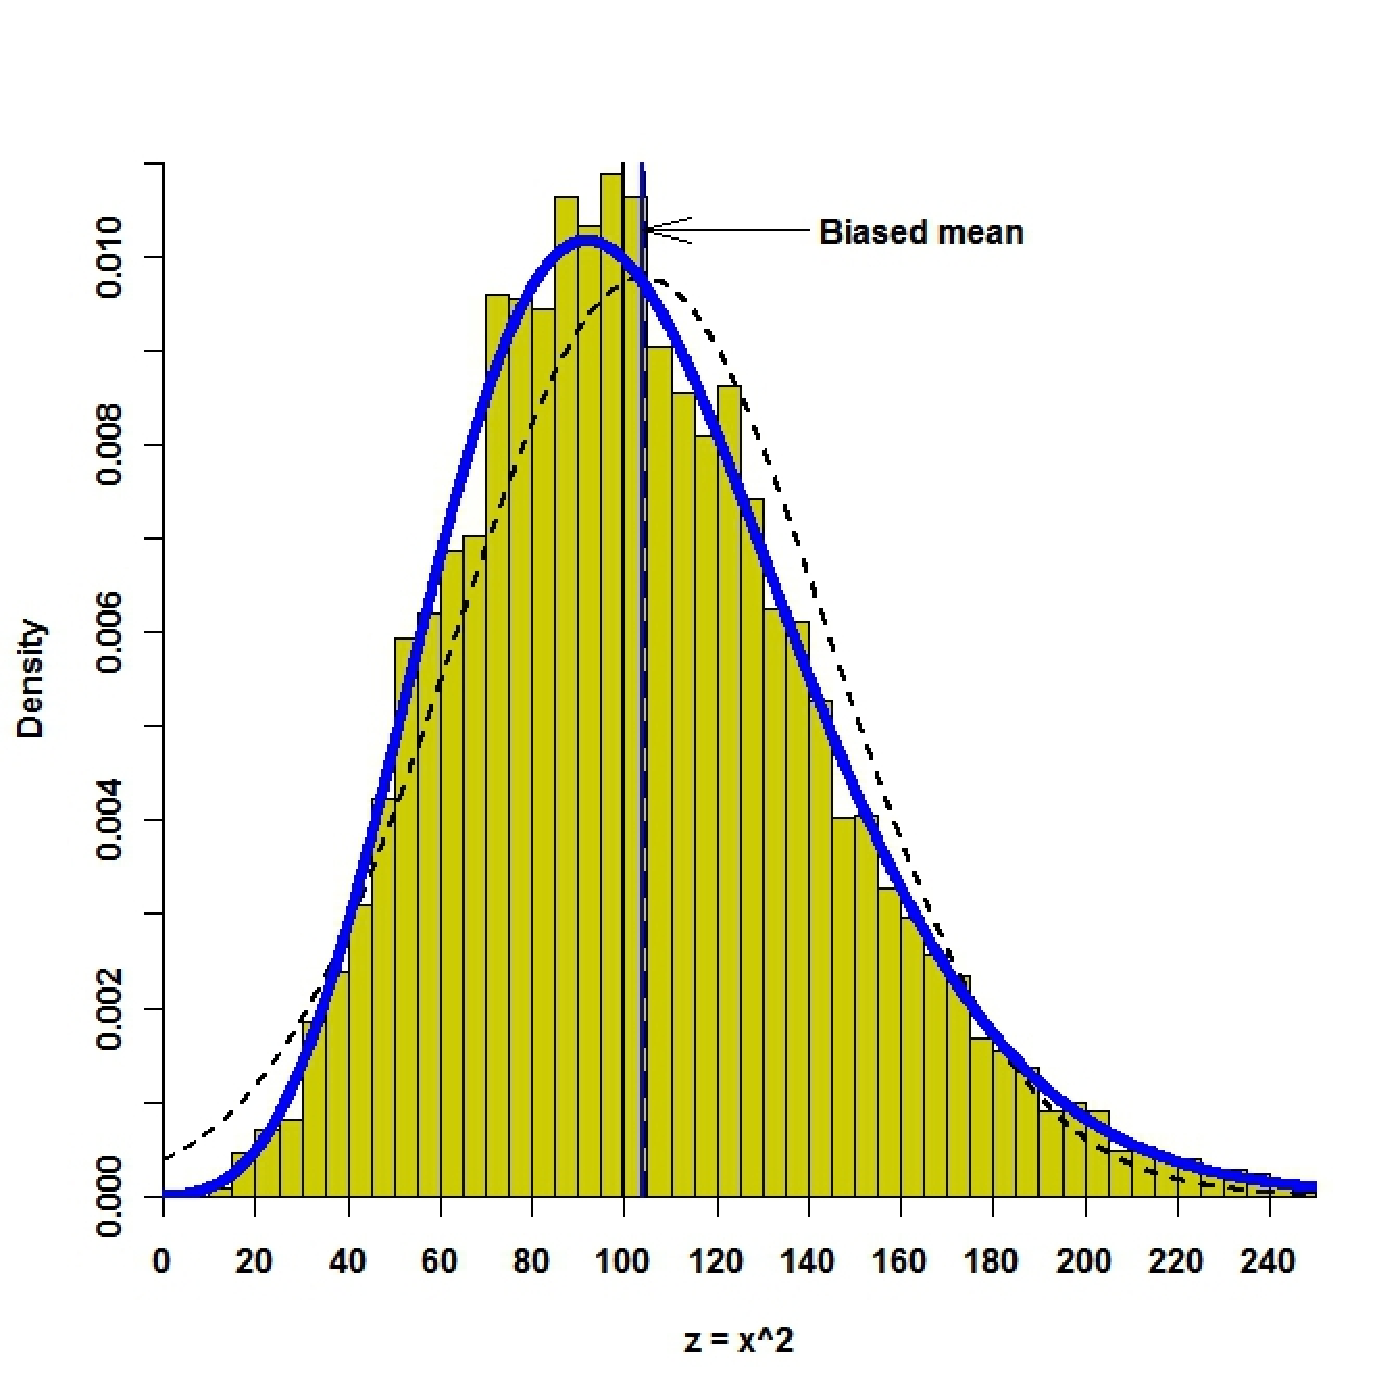
\includegraphics[scale=0.3]{hist} 
}

\frame{
  \frametitle{Sampling error, standard error}
\begin{itemize}
\item \textbf{Sampling error} or estimation error is the error caused by observing a sample instead of the whole population. 
\item The likely size of the sampling error can generally be controlled by taking a large enough random sample from the population
\item  If the observations are collected from a random sample, statistical theory provides probabilistic estimates of the likely size of the sampling error for a particular statistic or estimator. These are often expressed in terms of its \textbf{standard error}:
\[
m = \frac{\sigma }{\sqrt{N}}
\]
here $\sigma$ is standart deviation, $N$ -- number of observations
\end{itemize}
}

\frame{
  \frametitle{Correlation}
\begin{itemize}
\item In statistics, \textbf{correlation} and dependence are any of a broad class of statistical relationships between two or more random variables or observed data values.
\item The most familiar measure of dependence between two quantities is the \textbf{Pearson product-moment correlation coefficient}, or "Pearson's correlation." 
\[
 \mathbb{R}_{X,Y} = \frac{\mathrm{cov}(X,Y)}{\sigma_X \cdot \sigma_Y} = \frac{\sum\limits_{i=1}^n (x_i-\bar{x})(y_i-\bar{y})}{\sigma_X \cdot \sigma_Y}
\]
%  

\begin{center}
    \begin{tabular}{ | p{3cm}  | p{3cm}  |}
\hline
Correlation & $ \left | \mathbb{R}_{X,Y} \right |$ \\ \hline
None & 0.0 to 0.09 \\ \hline
Small & 0.1 to 0.3 \\ \hline
Medium & 0.3 to 0.5 \\ \hline
Large & 0.5 to 1.0 \\ \hline
 \end{tabular}
\end{center}
\end{itemize}
}
\frame{
  \frametitle{Correlation}
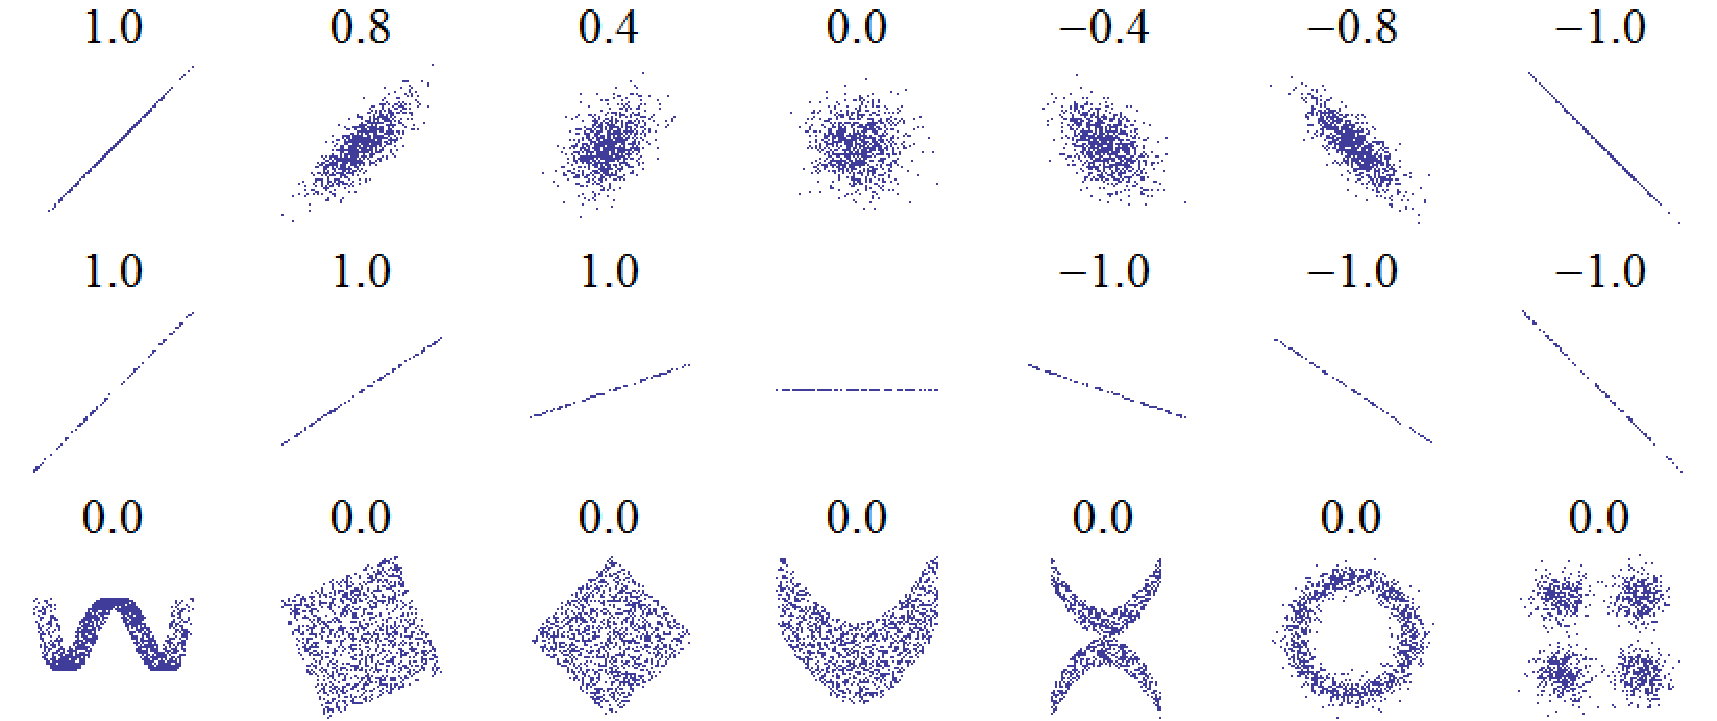
\includegraphics[scale=0.35]{cor}
}
% \frame{
%   \frametitle{Correlation - example}
% 
% }
\frame{
  \frametitle{Regression analysis}
\begin{itemize}
\item A method for fitting a curve (not necessarily a straight line) through a set of points using some goodness-of-fit criterion. 

\item The most common method for goodness-of-fit criteria -- \textbf{Least Squares Fitting}

\item The best fit in the least-squares sense minimizes the sum of squared residuals, a residual being the difference between an observed value and the fitted value provided by a model.
\end{itemize}

}
\frame{
  \frametitle{Regression analysis - example}
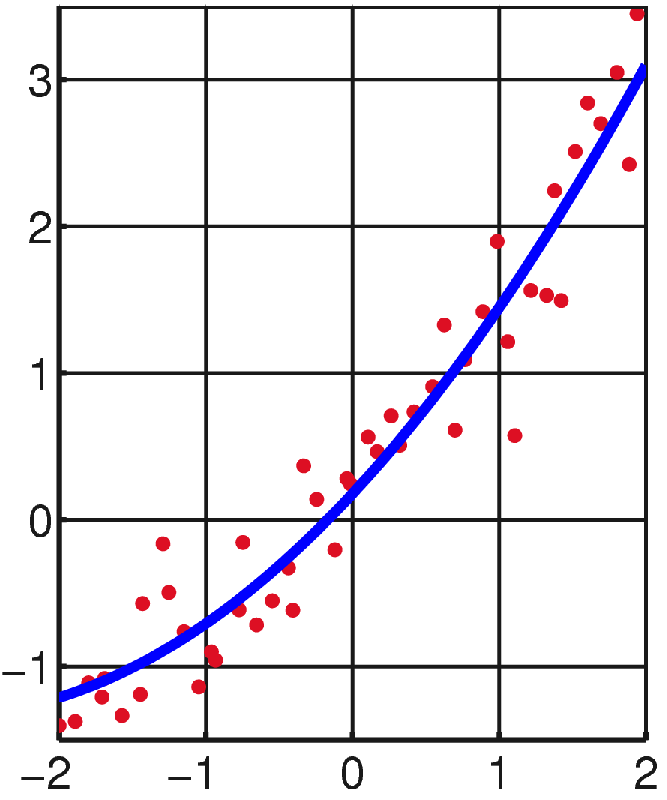
\includegraphics[scale=0.5]{ls} 
}

\frame{
  \frametitle{Post hoc ergo propter hoc}
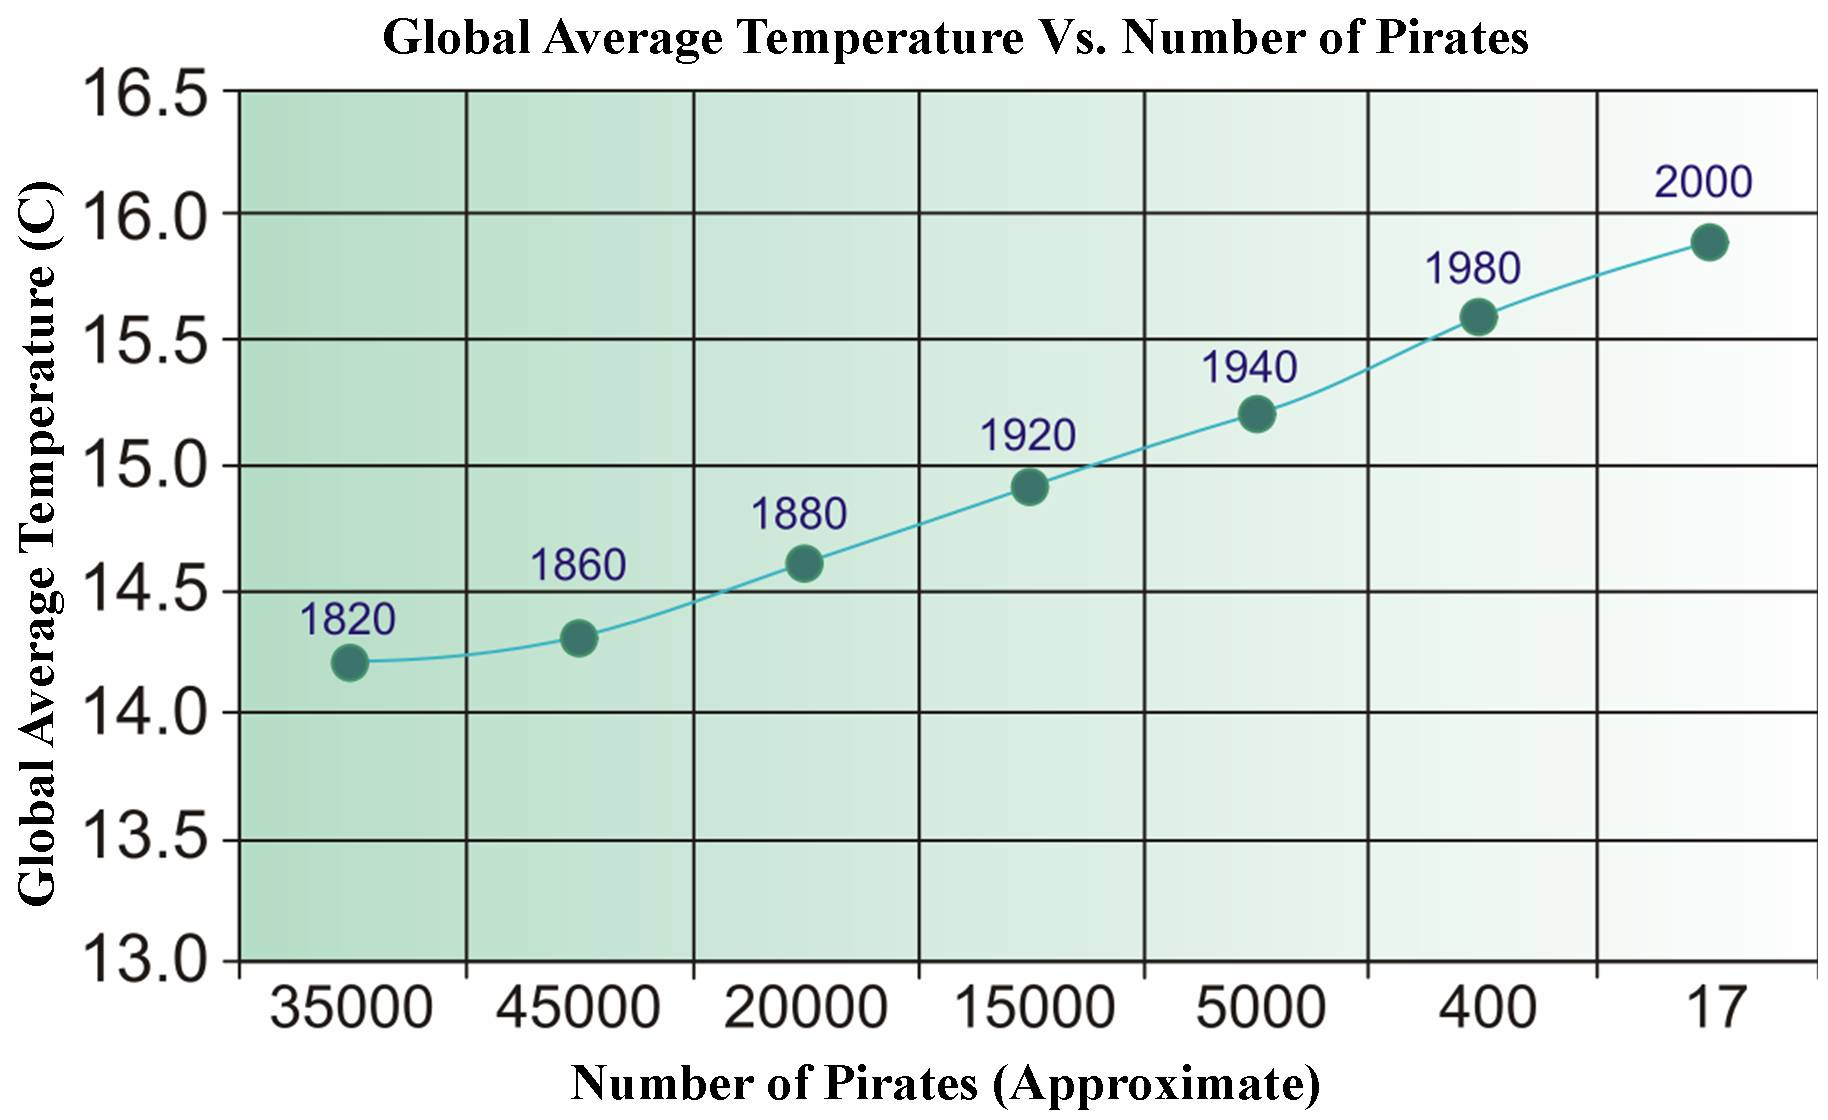
\includegraphics[scale=0.35]{pirates}
}
\frame{
  \frametitle{Post hoc ergo propter hoc}
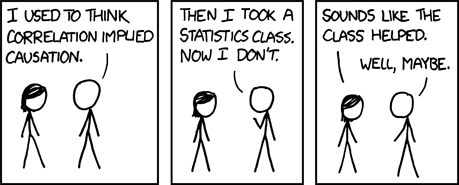
\includegraphics[scale=0.7]{correlation}
}

% \frame{
%   \frametitle{Statistical hypothesis testing}
% \begin{itemize}
% \item A statistical hypothesis test is a method of making decisions using data
%  \item A result is called \textbf{statistically significant} if it is unlikely to have occurred by chance alone, according to a pre-determined threshold probability, the \textbf{significance level}.
% \item A result that was found to be statistically significant is also called a \textbf{positive result}; conversely, a result whose probability under the null hypothesis exceeds the significance level is called a negative result or a null result.
% \end{itemize}
% }
% 
% \frame{
%   \frametitle{Type I error and Type II error}
% \begin{center}
%     \begin{tabular}{ | p{3cm}  | p{3cm}  | p{3cm}  |}
%     \hline
%      & Null Hypothesis ($H_{0}$) is true & Alternative Hypothesis ($H_{1}$) is true  \\ \hline
%      Fail to Reject Null Hypothesis & Right decision & Type II Error  \\ \hline
%      Reject Null Hypothesis & Type I Error &Right decision  \\ \hline
%     \end{tabular}
% \end{center}
% }
% 
% \frame{
%   \frametitle{Statistical hypothesis testing}
% \begin{itemize}
% \item We start with a research hypothesis of which the truth is unknown.
% \item The first step is to state the relevant null and alternative hypotheses. This is important as mis-stating the hypotheses will muddy the rest of the process. 
% \item The second step is to consider the statistical assumptions being made about the sample in doing the test; for example, assumptions about the statistical independence or about the form of the distributions of the observations.
% \item Decide which test is appropriate, and stating the relevant test statistic.
% \item Derive the distribution of the test statistic under the null hypothesis from the assumptions. 
% \item Compute from the observations the observed value tobs of the test statistic T.
% \item Decide to either fail to reject the null hypothesis or reject it in favor of the alternative. 
% \end{itemize}
% }
% \frame{
%   \frametitle{Pearson's $\chi^2$ test}
% 
% }
% \frame{
%   \frametitle{Pearson's $\chi^2$ test - algorithm}
% 
% }
% \frame{
%   \frametitle{Statistical hypothesis testing - example}
% 
% }
\frame{
\frametitle{Dixi}

\begin{center}
\Huge Dixi\end{center}
}
% \frame{
%   \frametitle{Dixi}
% \resizebox{.4\hsize}{!}{ Dixi }
% }
\end{document}
